\chapter[State of the Art]{State of the Art}

In this project, we focus on the operation of quantum simulators applied to molecular simulation, an area where quantum computing offers significant advantages. The main objective is to develop a program capable of simulating different molecules in a simple and efficient manner.

To this end, we will review the basic concepts of quantum mechanics that are essential to understand the fundamentals and potential of quantum computing, and explore the techniques of quantum simulation that allow us to harness quantum computing capabilities even with current technological limitations.

\section{Quantum Computing}

It is essential to understand the difference between bits in classical computing and qubits in quantum computing to delve into this new technological paradigm.

In classical computing, the basic unit of information is the \textbf{bit}, which can take the value of 0 or 1. These bits are the foundation upon which conventional computers operate, processing information through combinations of these binary states.

In contrast, quantum computing uses the \textbf{qubit} or quantum bit as its basic unit. Unlike the classical bit, a qubit can exist in a superposition of states, meaning it can simultaneously represent the values 0 and 1 thanks to the principle of superposition in quantum mechanics. This property, along with phenomena such as quantum entanglement and interference, allows quantum computers to process information exponentially more efficiently for certain problems.

\begin{figure}[H]
    \centering
    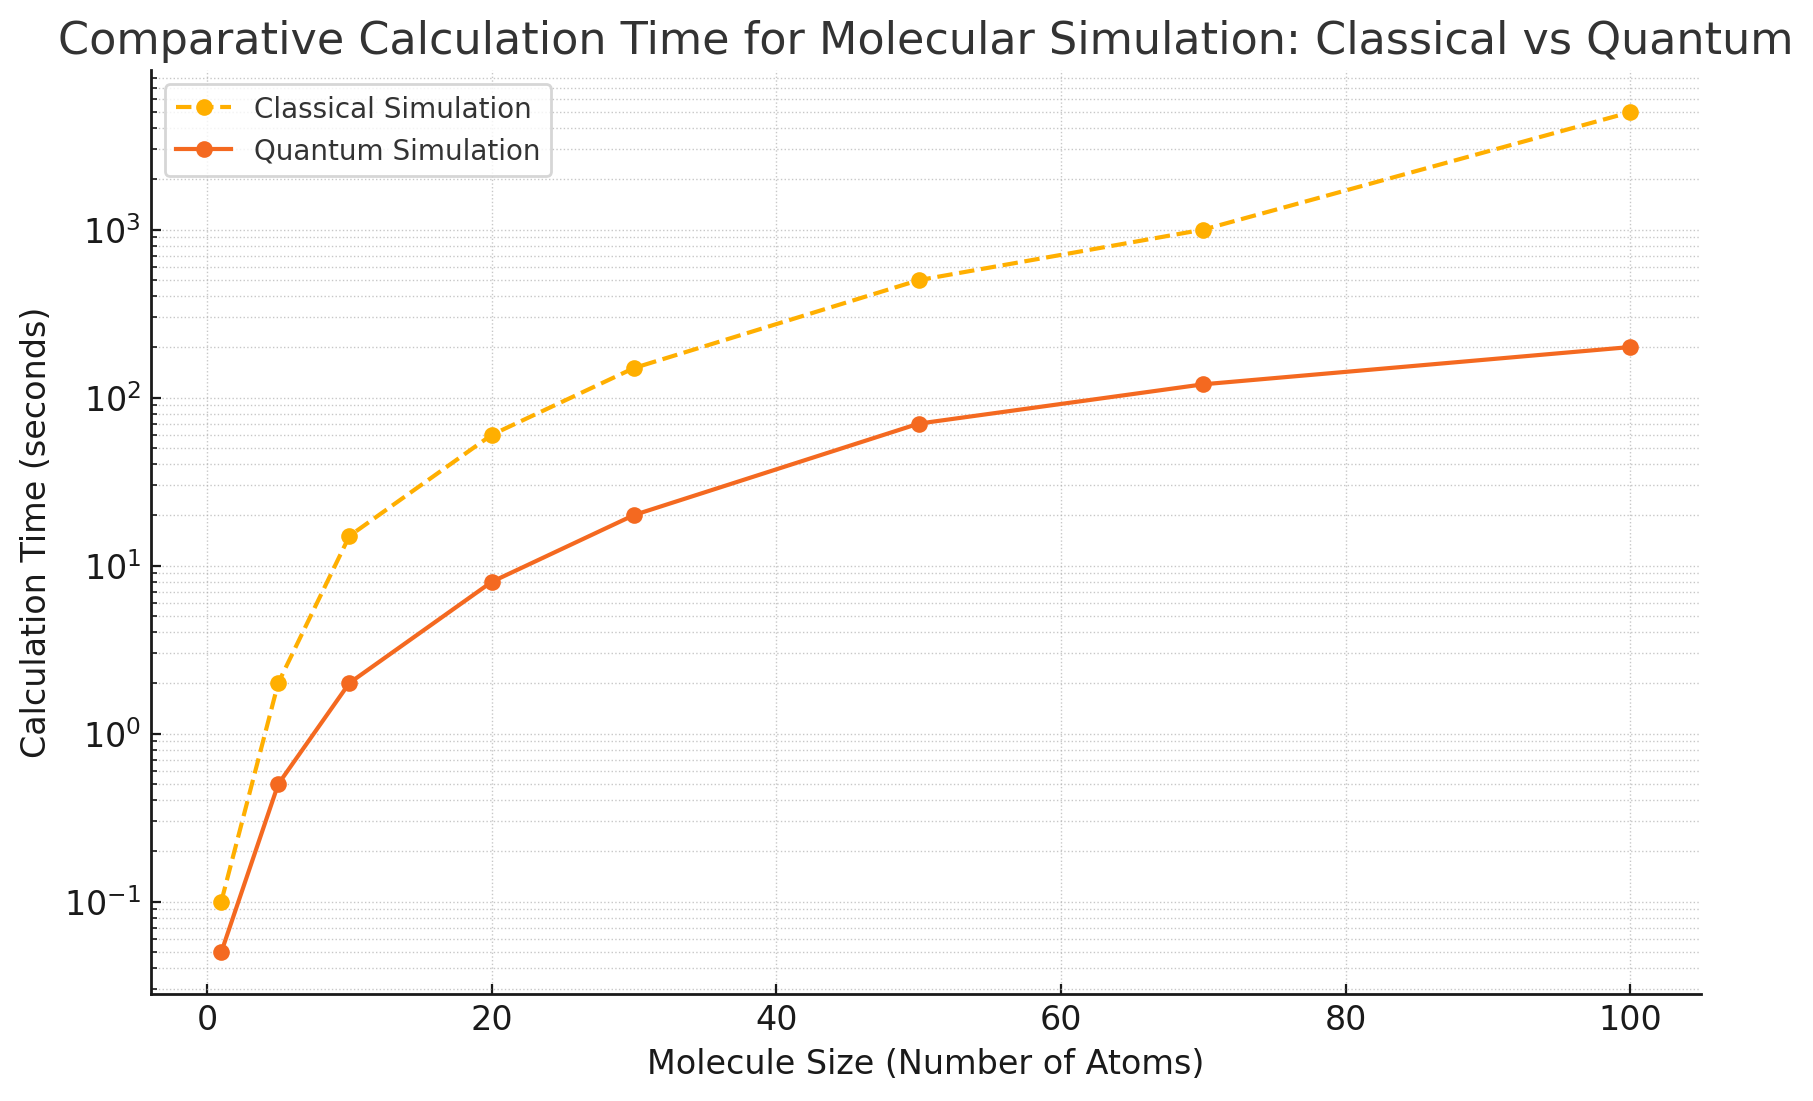
\includegraphics[width=0.8\textwidth]{img/bit_vs_qbit.png}
    \caption{Comparison between the growth of classical and quantum computational capacity.\cite{mooreslaw}}
    \label{fig:bit_vs_qubit}
\end{figure}

This graph shows us the boundaries that quantum computing allows us to reach compared to classical computing. It could achieve and dramatically surpass computational power.

Understanding how qubits operate and their differences from classical bits is essential to understand the potential of quantum computing. For this reason, the fundamental concepts of quantum computing are presented below.


\subsection{Qubit}

The \textbf{qubit} is the basic unit of information in quantum computing. While the classical bit can only be in one of two states (0 or 1), a qubit can be in a superposition of both states simultaneously. This is due to the principle of quantum superposition, one of the fundamental characteristics of quantum mechanics. It is worth noting that the states of a system are usually described by vectors, which reside in a Hilbert space.

For qubits, the Hilbert space is 2-dimensional, and the following values can be taken:

\begin{itemize}
    \item \(\ket{0}\): Represents the basis state 0.
    \[
    \ket{0} = \begin{pmatrix} 1 \\ 0 \end{pmatrix}
    \]

    \item \(\ket{1}\): Represents the basis state 1.
    \[
    \ket{1} = \begin{pmatrix} 0 \\ 1 \end{pmatrix}
    \]
\end{itemize}

Mathematically, a qubit is represented as a linear combination of the basis states $\ket{0}$ and $\ket{1}$:

\[
\ket{\psi} = \alpha\ket{0} + \beta\ket{1}
\]

where $\alpha$ and $\beta$ are complex numbers that satisfy the normalization condition $|\alpha|^2 + |\beta|^2 = 1$. These coefficients indicate the probability amplitudes of finding the qubit in the states $\ket{0}$ or $\ket{1}$ upon measurement.\cite{wikipedia_qubit}

\subsection{Quantum Entanglement}
An important distinguishing feature between qubits and classical bits is that multiple qubits can exhibit \textbf{quantum entanglement}; the qubit itself is an exhibition of quantum entanglement. In this case, quantum entanglement is a local or nonlocal property of two or more qubits that allows a set of qubits to express higher correlation than is possible in classical systems.

The simplest system to display quantum entanglement is the system of two qubits. Consider, for example, two entangled qubits in the \(\ket{\Phi^+}\) Bell state:
\[
\ket{\Phi^+} = \frac{1}{\sqrt{2}} \big( \ket{00} + \ket{11} \big).
\]
There are equal probabilities of measuring either product state \(\ket{00}\) or \(\ket{11}\), this is called \textbf{equal superposition}:
\[
\left| \frac{1}{\sqrt{2}} \right|^2 = \frac{1}{2}.
\]
In other words, there is no way to tell if the first and the second qubit has value 0 or 1.

To better understand quantum entanglement, let's explain an example. Imagine these qubits are separated, with one qubit given to Alice and the other to Bob. Alice performs a measurement, and the result she obtains has equal probabilities for both \(\ket{0}\) and \(\ket{1}\). If Bob measures the value of his qubit at the same time, the result must be exactly the same due to quantum entanglement.

If Alice's measurement had been \(\ket{0}\), then Bob's result would also have been \(\ket{0}\), because \(\ket{00}\) is the only state where Alice's qubit is \(\ket{0}\). In short, for these two entangled qubits, whatever Alice measures, so does Bob, demonstrating perfect correlation in any basis, regardless of the distance between them. This is a surprising phenomenon that cannot be explained by classical physics.\cite{pirandola2015advances}


\subsection{Quantum Superposition}

\textbf{Quantum superposition} allows a quantum system to exist in multiple states simultaneously until a measurement is performed. This characteristic is key to the functioning of quantum computers, as it enables processing a large amount of inputs simultaneously.

A qubit, by itself, is not much more powerful than a conventional bit. What makes it truly powerful is that it can place the quantum information it holds into a state of superposition, which represents a combination of all possible configurations of the qubit. Groups of qubits in superposition can create complex, multidimensional computational spaces, allowing complex problems to be represented in new ways within these spaces.\cite{ibm_quantum_computing}

Superposition is especially useful in simulating complex molecular systems. Quantum computers can naturally model the superpositions of electronic states in molecules, which is crucial for studying chemical reactions and molecular properties that are difficult to address with classical methods due to the exponential growth of computational resources required.

\subsection{Quantum Decoherence}

\textbf{Quantum decoherence} is one of the main challenges in quantum computing. Such machines are expected to rely heavily on the undisturbed evolution of quantum coherence. Decoherence causes the system to lose its quantumness, which invalidates the superposition principle and turns quantum to classical behavior. They must handle the decoherence in order to maintain quantum computation performance.\cite{optimizing_decoherence}

Qubits are extremely sensitive to external disturbances, such as electromagnetic fluctuations, vibrations, and temperature changes. These interactions can cause quantum states to mix with those of the environment, leading to a loss of coherence that is irreversible and degrades the stored quantum information.\cite{decoherence}

To mitigate the effects of decoherence, various strategies are implemented:

\begin{itemize}
    \item \textbf{System Isolation}: Designing physical systems that minimize unwanted interactions with the environment, using materials and techniques that protect qubits from external disturbances.
    \item \textbf{Quantum Error Correction}: Implementing error correction codes that allow detecting and correcting errors without directly measuring the qubit's state, thereby preserving quantum information.
    \item \textbf{Dynamic Control}: Applying techniques such as pulse refocusing and dynamic pulse sequences that actively compensate for disturbances and extend the coherence time of qubits.
\end{itemize}

Controlling and mitigating decoherence are essential for the advancement of quantum computing and its application in areas like molecular simulation, where the precision of calculations is fundamental.


\section{Quantum Simulation}

Quantum simulation has become a vital tool for investigating intricate quantum systems that are beyond the reach of classical computational methods. Building on Richard Feynman’s idea that a computer operating on quantum principles could exceed the capabilities of classical machines for modeling quantum behavior, the field has seen rapid advancements. Today, it spans both digital and analog approaches and finds applications in numerous scientific domains.

There are mainly two approaches in quantum simulation: \textbf{Digital Quantum Simulation (DQS)} and \textbf{Analog Quantum Simulation (AQS)}. DQS employs quantum circuit models to study the dynamics of the system, thus emulating, with the help of qubits, the behavior of the system. This approach is universal, as it can, in principle, simulate any quantum system, although not always efficiently. On the other hand, AQS uses an accessible quantum system to emulate the Hamiltonian of the system, thereby allowing us to learn about the properties of the system we want to study. This method is particularly useful when a qualitative representation is required rather than high precision.\cite{AQS}

In addition to these approaches, there are algorithms inspired by quantum information theory that facilitate the classical simulation of quantum systems using the internal symmetries of particles. Techniques such as \textbf{Matrix Product States (MPS)} and \textbf{Projected Entangled Pair States (PEPS)} allow representing particle systems on classical computers more efficiently than standard classical methods, optimizing the calculation of properties of complex quantum systems.
\cite{mps_peps_tensor_networks}

The applications of the quantum simulation systems are an exciting area of scientific practice. In condensed matter physics, it allows the study of models such as the Hubbard model and quantum phase transitions, fundamental for understanding phenomena like superconductivity, it facilitates the calculation of molecular energies and complex chemical reactions, it emulates particles in high-energy fields and cosmological phenomena. Furthermore, quantum simulation promises to have applications in the study of many problems; high-energy physics, atomic physics, quantum chemistry, condensed-matter physics and cosmology. This could be implemented using quantum computers, but also with
simpler, analog devices that require less control and are, therefore, easier to construct.\cite{QuantumSimulation}

But there are still challenges to deal with. It’s tough to control quantum simulator systems properly. Plus, errors and decoherence can degrade or adversely affect the results. The number of qubits and quantum gates we need depends on how big and complex the system is. We think you need around 40 to 100 qubits to beat classical computers on some problems. Despite these hurdles, tech is advancing, and we’re getting better at quantum simulation. This could really change how we do research in science and help us learn more about the quantum world.

\section{Hamiltonian}

The Hamiltonian is a fundamental concept originating from classical mechanics, who developed a reformulation of Newtonian mechanics. Hamiltonian mechanics is a reformulation of classical mechanics that provides powerful tools for studying the dynamics of systems. 

The Hamiltonian of a system represents the total energy of the system, expressed in terms of generalized coordinates and momenta, and is given by the sum of the kinetic and potential energies. The \textbf{Hamiltonian operator} plays a central role in describing the energy and time evolution of quantum systems, takes different forms and can be simplified, in some cases. It represents the total energy of the system, including kinetic and potential energies, being essential for formulating the Schrödinger equation.\cite{wiki:hamiltonian_quantum_mechanics}

\subsection{Mathematical Definition}

The Hamiltonian operator, typically denoted as \( \hat{H} \), is a self-adjoint operator acting on the Hilbert space associated with the quantum system. For a single particle in one dimension, the Hamiltonian is expressed as:

\[
\hat{H} = \hat{T} + \hat{V}
\]

where:

\begin{itemize}
    \item \( \hat{T} \) is the kinetic energy operator.
    \item \( \hat{V} \) is the potential energy operator.
\end{itemize}

In terms of the position \( \hat{x} \) and momentum \( \hat{p} \) operators, these are defined as:

\[
\hat{T} = \frac{\hat{p}^2}{2m} = -\frac{\hbar^2}{2m} \frac{d^2}{dx^2}
\]

\[
\hat{V} = V(\hat{x})
\]

Here, \( m \) is the mass of the particle, \( \hbar \) is the reduced Planck constant, and \( V(\hat{x}) \) is the potential energy function depending on position.

Finally, it can be shown that the expectation value of the Hamiltonian, which represents the energy expectation value, is always greater than or equal to the system's minimum potential:\cite{wiki:hamiltonian_quantum_mechanics}

Computing the expectation value of the kinetic energy, we have:
\[
\begin{aligned}
T &= -\frac{\hbar^2}{2m} \int_{-\infty}^{+\infty} \psi^* \left( \frac{d^2 \psi}{dx^2} \right) \, dx \\ 
  &= -\frac{\hbar^2}{2m} \left( \left[ \psi'(x) \psi^*(x) \right]_{-\infty}^{+\infty} 
      - \int_{-\infty}^{+\infty} \left( \frac{d\psi}{dx} \right) 
      \left( \frac{d\psi}{dx} \right)^* \, dx \right) \\ 
  &= \frac{\hbar^2}{2m} \int_{-\infty}^{+\infty} \left| \frac{d\psi}{dx} \right|^2 \, dx \geq 0.
\end{aligned}
\]
Hence the expectation value of the kinetic energy is always non\-negative. We can calculate the expectation value of the total enegy for normalized wavefunction:

\[
E = T + \langle V(x) \rangle = T + \int_{-\infty}^{+\infty} V(x) |\psi(x)|^2 \, dx 
\geq V_{\text{min}}(x) \int_{-\infty}^{+\infty} |\psi(x)|^2 \, dx \geq V_{\text{min}}(x).
\]


\subsection{Role in the Schrödinger Equation}

The Hamiltonian is central to the Schrödinger equation, which describes how the quantum state of a system evolves over time. The time-dependent Schrödinger equation is expressed as:

\[
i\hbar \frac{\partial}{\partial t} |\psi(t)\rangle = \hat{H} |\psi(t)\rangle
\]

where \( |\psi(t)\rangle \) is the state vector of the system at time \( t \). For time-independent systems, the Schrödinger equation reduces to the eigenvalue equation:

\[
\hat{H} |\psi\rangle = E |\psi\rangle
\]

Here, \( E \) represents the energy level or eigenvalues of the state $\psi$ , this equation is known as the \textit{time-intependent Schrödinger equation}.\cite{tao_schrodinger}

\subsection{Hamiltonian in Multi-Particle Systems}

We can extend the concept of the Hamiltonian to systems with N particles.\cite{wiki:hamiltonian_quantum_mechanics} The Hamiltonian is expressed as:

\[
\hat{H} = \sum_{n=1}^{N} \hat{T}_{n} + \hat{V}
\]

where:
\begin{itemize}
    \item \(\hat{V}\): is the potential energy function, which depends on the spatial configuration of the system and time. A particular set of spatial positions at a given instant defines a configuration.
    \item \(\hat{T}_{n}\): is the kinetic energy operator for particle \(n\), given by:
    \[
    \hat{T}_{n} = \frac{\mathbf{\hat{p}}_{n} \cdot \mathbf{\hat{p}}_{n}}{2m_{n}} = -\frac{\hbar^2}{2m_{n}} \nabla_{n}^2
    \]
\end{itemize}

Combining these yields, the Schrödinger Hamiltonian for an N number of particles system:
\[
\begin{aligned}
\hat{H} &= \sum_{n=1}^{N} \hat{T}_{n} + \hat{V} \\[6pt]
        &= \sum_{n=1}^{N} \frac{\mathbf{\hat{p}}_{n} \cdot \mathbf{\hat{p}}_{n}}{2m_{n}} + V(\mathbf{r}_{1}, \mathbf{r}_{2}, \ldots, \mathbf{r}_{N}, t) \\[6pt]
        &= -\frac{\hbar^2}{2} \sum_{n=1}^{N} \frac{1}{m_{n}} \nabla_{n}^2 + V(\mathbf{r}_{1}, \mathbf{r}_{2}, \ldots, \mathbf{r}_{N}, t)
\end{aligned}
\]
\subsection{The second quantization}

Finding an exact solution of the  Schrödinger equation is equivalent to solving the Full Configuration Interaction (FCI) functions, where the wave function of a molecule is represented as a sum of all possible Slater determinants that can be formed using a specific set of molecular orbitals. As the number of electrons and orbitals increases, the number of Slater determinants grows exponentially, making the FCI method computationally infeasible for large systems. Therefore, it is recommended to use a quantum computer to solve this problem. For this reason, we need to transform the Hamiltonian to the second quantized operators' form.

For more than one particle, the second\-quantized Hamiltonian can be written under the form:
\[
H =
\sum_{p,q} h_{pq} a_p^\dagger a_q +
\sum_{p,q,r,s} h_{pqrs} a_p^\dagger a_q^\dagger a_r a_s,
\]
with \(a^\dagger\) and \(a\) being the electron creation and annihilation operators. The first term thus represents the transitions of single electrons between orbitals, while the second term corresponds to the interactions between pairs of electrons\cite{SecondQuantization}.

\subsection{Importance in Quantum Simulations}

In quantum simulations, especially in algorithms like the Variational Quantum Eigensolver (VQE), the Hamiltonian is decomposed into a sum of simpler terms, often expressed in terms of Pauli operators. This decomposition facilitates implementation on quantum circuits and allows estimating the system's energy through measurements on qubits.

Understanding the structure and properties of the Hamiltonian is essential for modeling and simulating quantum systems, as it determines the possible energies and dynamics of the system under study.

\section{VQE: Variational Quantum Eigensolver}
\label{sec:vqe}

Variational quantum eigensolvers (VQEs) are among the most promising candidates for achieving useful computations in chemistry on near-term quantum computers. They operate by varying parameters and optimizing them to achieve the lowest energy, this can be achived by using variational principle from quantum mechanics. 

At their core, they prepare a quantum state, determined by a set of classical parameters that are specified by an \textit{ansatz}, measuring its energy on the quantum computer. Then, a new quantum state is prepared with a new set of parameters, selected by any classical optimization algorithm, and the process is repeated until the energy is minimized. If the energy is carried out perfectly, we approximate this value to the ground-state energy. \cite{VQEs}

Among the hybrid quantum-classical algorithms developed to address quantum simulation challenges, the \emph{Variational Quantum Eigensolver (VQE)} has gained particular relevance. That aims to solve for the ground state of a given Hamiltonian represented as a linear combination of Pauli terms, with an ansatz circuit where the number of parameters to optimize over is polynomial in the number of qubits. \cite{ibm_vqe_tutorial}

\subsection{Fundamental Principles and Stages of the Algorithm}
\label{subsec:vqe_principles_stages}

VQE is founded on the \textbf{variational principle} of quantum mechanics, which states that the expectation value of the energy 
\(\,E(\vec{\theta})\)
for any normalized trial state \(\,\ket{\psi(\vec{\theta})}\) is always an upper bound to the true ground-state energy \(E_0\):
\[
E(\vec{\theta}) 
= \bra{\psi(\vec{\theta})} \hat{H} \ket{\psi(\vec{\theta})}
\;\;\geq\; E_0.
\]

Because \(E(\vec{\theta})\) depends on a set of parameters \(\vec{\theta}\), the VQE iteratively updates these parameters to minimize the resultant energy. Once no further reduction in \(E(\vec{\theta})\) is possible, the algorithm identifies that we reached the best approximation of \(E_0\).
\begin{figure}[H]
    \centering
    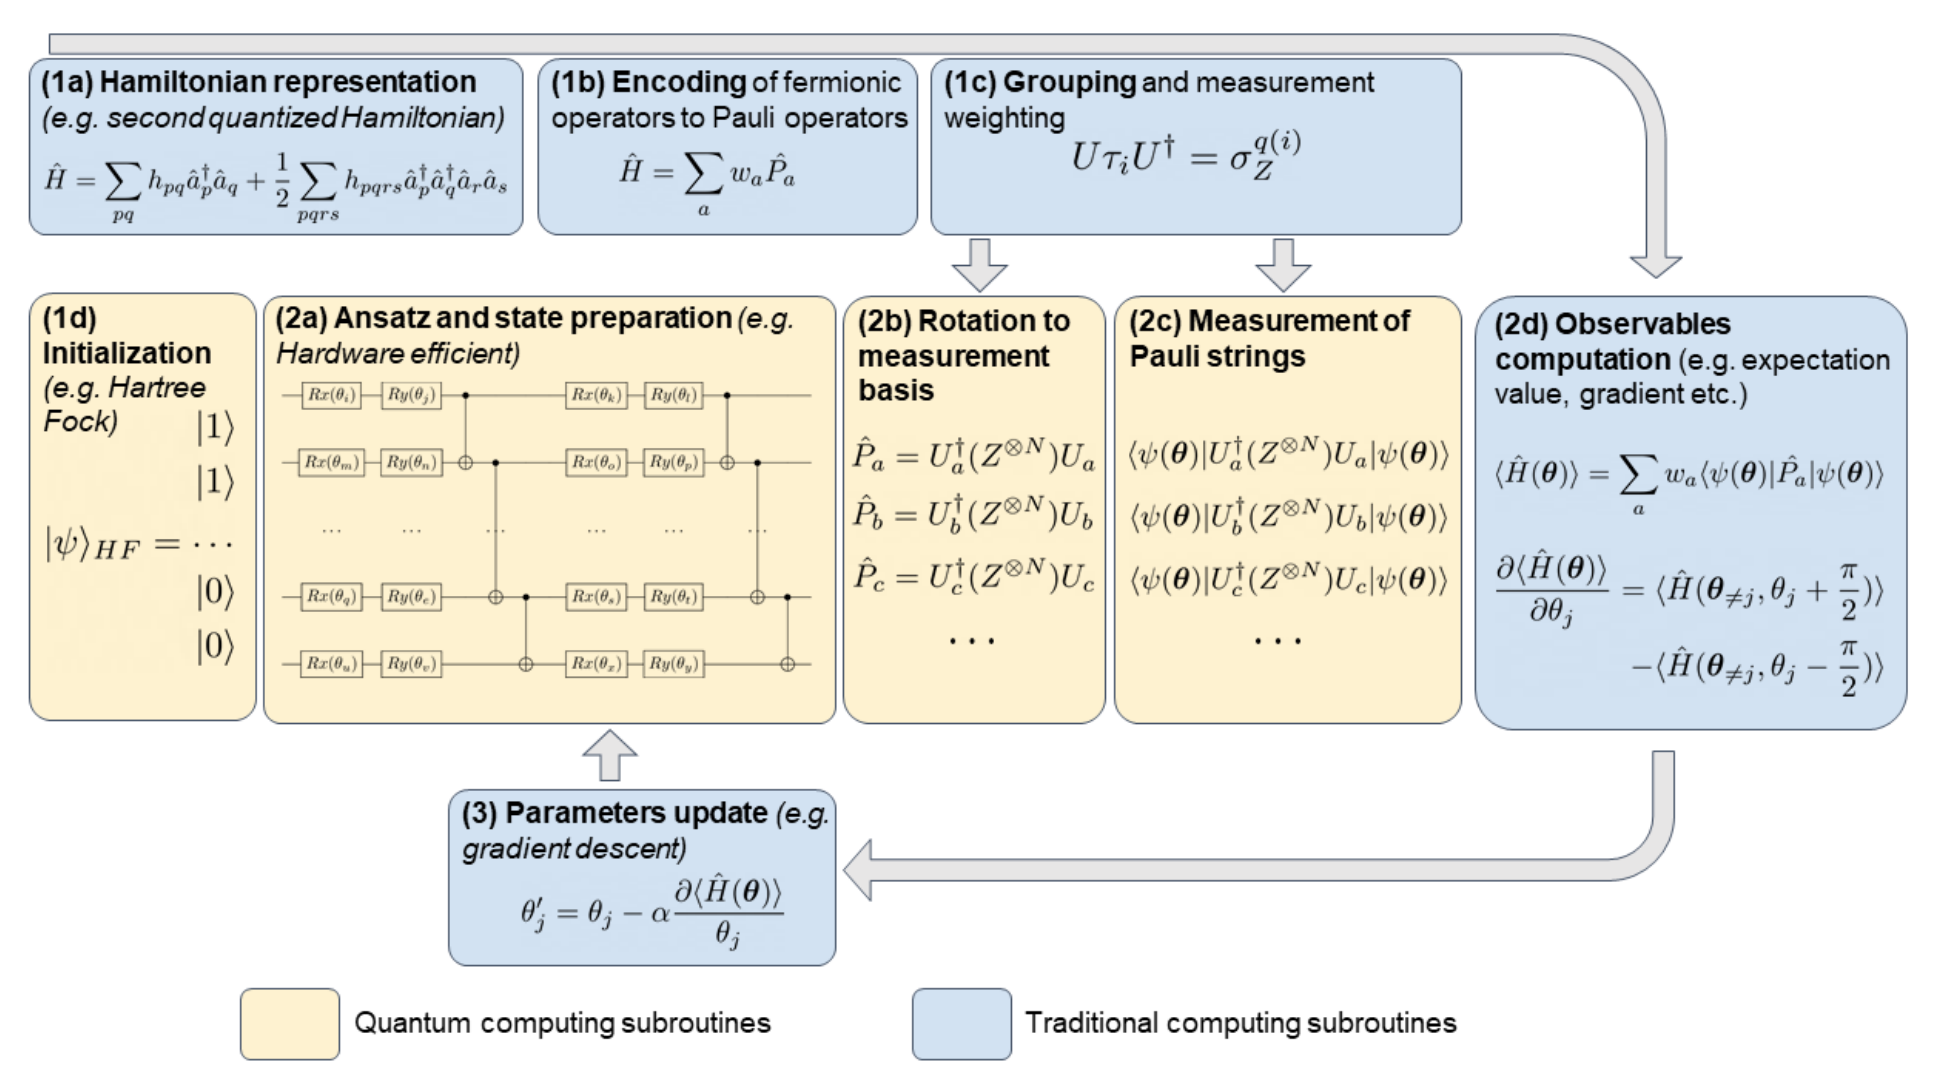
\includegraphics[width=0.8\textwidth]{img/VQE_flowchart.png}
    \caption{VQE pipline\cite{VQE_review}.}
    \label{fig:vqe_flowchart}
\end{figure}

In this image, we find a flowchart of a VQE algorithm. Below, we describe the steps of the algoritm:


\begin{enumerate}
    \item \textbf{Hamiltonian Construction and representation:} 
    The first step of the algorithm is define the sytem for which we want to calculate the ground state. For that, we construc the Hamiltonian of the system. Constructing the Hamiltonian involves finding specific operators with their own weights.
    
    \item \textbf{Encoding of operators:}
    The next step, is to encode Hamiltonian operators, on quantum computers, we can only measure observables expressed in Pauli basis, due to the two-lavel nature of qubits. In first quantization, the operators can be directly translated into spin operators. In second quantization, the operators are expressed as a linear combination of fermionic operators.

    \item \textbf{Measurement of the Expected Energy:}
    The expectation value 
    \(\langle \psi(\vec{\theta}) \mid \hat{H} \mid \psi(\vec{\theta}) \rangle\)
    is obtained by measuring the appropriate Pauli operators on the quantum device, typically requiring multiple circuit executions due to non-commuting terms.

    \item \textbf{Ansatz and State Preparation:}
    Once we have prepared the Hamiltonian such that we can measure his expectation value on a quantum device, we can proceed to the preparation of the wavefunction. To achieve this, we need to decide the parametrized quantum circuit, denoted as ansatz. One of the main aspects that we have to take into account, is that the ansatz must be sufficiently expressive to guarantee that it can appropriately aproximate the ground state wavefunction.

    \item \textbf{Parameter Optimization:}
    Finally, the parameters of the ansatz used need to be updated iteratively until convergance. The measured energy serves as a cost function, we repeat the process until the convergence criteria is achieved.

    We can define the convergence criteria as:
    \[
    \left|\,E\bigl(\vec{\theta}_{k+1}\bigr) - E\bigl(\vec{\theta}_{k}\bigr)\right|
    \;<\;\delta,
    \]
    where \(\delta\) is a small threshold for energy differences. The final set \(\vec{\theta}^{*}\) yields an approximate ground-state wavefunction and energy.
\end{enumerate}

\subsection{Advantages and Challenges}
\label{subsec:vqe_challenges}

VQE has garnered extensive interest in fields like \textbf{quantum chemistry}, \textbf{materials science}, and even combinatorial optimization problems mapped to Hamiltonians. Its hybrid structure allows leveraging near-term quantum devices (with limited qubits and gate depths) while offloading resource-intensive tasks---such as parameter updates---to classical computers. 

Despite its promise, VQE faces several practical challenges:

\begin{itemize}
    \item \textbf{Noise and Decoherence:} 
    Real quantum devices suffer from errors that deteriorate the fidelity of prepared states and measurements, requiring error-mitigation strategies and noise-aware ansatz designs.

    \item \textbf{Barren Plateaus:}
    High-dimensional parameter spaces can contain large regions where gradients vanish, complicating the search for global minima.

    \item \textbf{Measurement Overhead:}
    Decomposing a Hamiltonian into many Pauli terms demands running multiple circuits, increasing sampling time and exposure to hardware noise.

    \item \textbf{Circuit Depth:}
    Accurate ans\"atze for complex systems may require deep circuits that quickly exceed the coherence times of current quantum processors.
\end{itemize}

\subsection{Outlook in Quantum Simulation}
\label{subsec:vqe_outlook}

Continuous improvements in hardware (qubit quality, gate fidelity, and error-correction schemes) and software (advanced ans\"atze, better optimizers, error mitigation) keep driving VQE toward practical applications. Recent strategies such as \emph{ADAPT-VQE}\cite{ADAPTVQE}, which determines a quasi-optimal ansatz with the minimal number of operators necessary to achieve the desired accuracy. The key idea is to systematically add fermionic operators one\-at\-a\-time, such that the maximal amount of correlation energy is captured at each step.

As the number of qubits grows and quantum hardware evolves, VQE is likely to become a central approach for tackling classically intractable problems in quantum chemistry, materials science, and beyond. Its flexible hybrid nature will continue to serve as a testbed for new optimization algorithms, ansatz designs, and measurement strategies, bridging current \emph{Noisy Intermediate-Scale Quantum (NISQ)} devices with the longer-term ambition of fault-tolerant quantum computing.

\section{Ans\"{a}tze}
In the context of variational quantum algorithms and quantum chemistry, an \textbf{ansatz} is a carefully chosen, often physically motivated, parametric form of the quantum state used to approximate the ground state of a system described by a given Hamiltonian. The term \textit{ansatz} originates from the German word \textquotedblleft approach\textquotedblright\ or \textquotedblleft initial guess,\textquotedblright\ and it reflects the central idea that we propose a functional form for the wavefunction and then we optimize the parameters in search of the lowest possible energy. 

Within the framework of the Variational Quantum Eigensolver (VQE), the ansatz is implemented as a parameterized quantum circuit whose gates depend on a set of continuous variables $\vec{\theta}$. It is used to produce the trial state, with which the Hamiltonian can be measured to obtain an estimate energy, $E(\vec{\theta})$, which is then iteratively minimized by a classical optimizer. The key aspects of the ansatz are the expressiveness and trainability of the chosen ansatz. The expressibility is the ability of the ansatz to span a large class of states, while the trainability describes the practical ability of the ansatz to be optimized using techniques tractable on quantum devices 
in the Hilbert space. 

Several ans\"{a}tze have been proposed to achieve a balance between accuracy and computational cost. Below, we summarize the most relevant approaches, highlighting their theoretical underpinnings and current usage in quantum simulation\cite{VQE_review}.

\subsection{Hartree--Fock-based Ans\"{a}tze (Classical Reference)}
A historically important \textquotedblleft classical\textquotedblright\ ansatz in quantum chemistry arises from the \textbf{Hartree--Fock (HF)}\cite{wiki:hartree_fock_method} approximation. In this method, the total wavefunction is assumed to be a single Slater determinant constructed from one-particle orbitals. Although it captures the fundamental antisymmetry required by the Pauli exclusion principle, it neglects most of the electron correlation. Post-HF methods, such as Configuration Interaction (CI), Many-Body Perturbation Theory (MPn), and Coupled Cluster (CC), then build on this reference state by introducing additional terms that account for electron correlation.\cite{wiki:post_hartree_fock}  

\begin{itemize}
    \item \textbf{Configuration Interaction (CI):} Expands the wavefunction in a basis of Slater determinants (excitations) beyond the HF reference. The Full CI approach is exact within the chosen basis but scales exponentially with system size. Truncated CI methods (CIS, CID, CISD, etc.) reduce the computational cost but still grow quickly with system size.

    \item \textbf{Coupled Cluster (CC):} CC is a post Hartree-Fock method that aims at recovering a portion of electron correlation energy by evolving an initial wave function (usually the Hartree-Fock wave function) under the action of parametrized excitation operators. Formally written as 
    \[
       |\Psi_{\mathrm{CC}}\rangle = e^{\hat{T}}|\Phi_{\mathrm{HF}}\rangle,
    \]
    where $\hat{T}$ is the sum of cluster excitation operators (singles, doubles, triples, etc.). Although Coupled Cluster with Singles and Doubles (CCSD) is often accurate, further inclusion of triples and higher excitations can be required for strongly correlated systems.
\end{itemize}

In the context of classical methods, these \textbf{ans\"{a}tze} serve as trial wavefunctions whose coefficients are optimized using high-performance classical algorithms. Their conceptual basis---constructing physically motivated trial states that capture crucial features of the system---carries over into quantum computing.

\subsection{Unitary Coupled Cluster (UCC)}
A key adaptation of the Coupled Cluster theory to quantum computing is the \textbf{Unitary Coupled Cluster (UCC)} ansatz. It modifies the standard CC exponential by making it explicitly unitary:

\[
|\Psi_{\mathrm{UCC}}\rangle 
= e^{\hat{T}(\vec{\theta}) - \hat{T}^\dagger(\vec{\theta})} \,|\Phi_{\mathrm{HF}}\rangle,
\]

where $\hat{T}(\vec{\theta})$ is typically truncated to include only single and double excitations (UCCSD). This approach guarantees that the resulting operator is unitary, which is crucial for hardware implementations in quantum computing since all gates must be unitary transformations. 

\begin{itemize}
    \item \textbf{UCCSD (Singles and Doubles):} The most widespread version of UCC is truncated at single and double excitations:
    \[
        \hat{T}(\vec{\theta}) = \sum_{i,a} \theta_{i}^{a} \hat{a}_a^\dagger \hat{a}_i 
          \,\,+\,\, 
          \sum_{i,j,a,b} \theta_{i,j}^{a,b} \hat{a}_a^\dagger \hat{a}_b^\dagger \hat{a}_j \hat{a}_i
          \,\,+\, \cdots
    \]
    Here, $i, j$ denote occupied orbitals and $a, b$ virtual (unoccupied) orbitals. By exponentiating both $\hat{T}$ and $\hat{T}^\dagger$, the wavefunction stays normalized. However, the circuit depth can become large since implementing the exponential of a sum of non-commuting operators requires a trotterization or related approximation.

    \item \textbf{ADAPT-VQE and Variants:} To mitigate the high circuit cost, variants like \textit{ADAPT-VQE} build up a UCC-type ansatz incrementally, selecting only those excitation operators that most significantly lower the energy at each step. This adaptive approach reduces the number of gates needed and often converges faster.
\end{itemize}

\section{Optimizers}
\label{sec:optimizers}

In quantum simulation algorithms such as the Variational Quantum Eigensolver (VQE), optimizers constitute a key element of the hybrid quantum-classical workflow. Their primary objective is to minimize the cost function
\[
E(\vec{\theta}) = \langle \psi(\vec{\theta}) \mid \hat{H} \mid \psi(\vec{\theta}) \rangle,
\]
where \(\hat{H}\) represents the Hamiltonian of the system under study and \(\ket{\psi(\vec{\theta})}\) is a parameterized quantum state, often referred to as the \emph{ansatz}. After each quantum measurement, the optimizer updates the parameter vector \(\vec{\theta}\) to guide the system toward the ground-state energy. This process is iterated until convergence, balancing the capabilities of quantum hardware with classical numerical techniques.

In the following subsections, we are going to describe, all the optimizers used in this project. While all these optimizers share the goal of efficiently navigating the parameter space, they differ in how they incorporate gradients, memory of past iterations, and adjustments of the learning rate.\cite{OptimizationAlgorithms} 

\subsection{Gradient Descent (GD)}
\label{subsec:gd}
\emph{Gradient Descent} is one of the most fundamental methods for continuous optimization. At each iteration, it updates parameters by moving them in the direction opposite to the gradient of the cost function:
\[
\vec{\theta}_{k+1} = \vec{\theta}_{k} 
- \eta \nabla_{\vec{\theta}} E(\vec{\theta}_{k}),
\]
where \(\eta\) is the learning rate and \(\nabla_{\vec{\theta}} E(\vec{\theta})\) denotes the gradient of the cost function with respect to the parameters. Gradient Descent can converge slowly or get trapped in local minima when dealing with complex or high-dimensional landscapes, making it less efficient if used alone in large-scale molecular simulations.

\subsection{Momentum Optimizer}
\label{subsec:momentum}
The \emph{Momentum} method extends standard Gradient Descent by incorporating a velocity term that accumulates a fraction of previous updates. This approach can mitigate oscillations and speed up convergence in regions with shallow gradients. The update rule is given by:
\[
\begin{aligned}
\vec{v}_{k+1} &= \gamma \vec{v}_{k} 
+ \eta \nabla_{\vec{\theta}} E(\vec{\theta}_{k}),\\
\vec{\theta}_{k+1} &= \vec{\theta}_{k} - \vec{v}_{k+1},
\end{aligned}
\]
where \(\gamma\) (typically between 0.9 and 0.99) is the momentum coefficient that controls how much past gradients influence the current update. This optimizer often accelerates learning in practice by effectively smoothing noisy or rapidly changing gradients.

\subsection{Nesterov Momentum Optimizer (NMomentum)}
\label{subsec:nmomentum}
\emph{Nesterov Momentum}, sometimes referred to as \emph{Nesterov’s Accelerated Gradient (NAG)}, refines the idea of Momentum by anticipating the next position of the parameters before computing the gradient. Concretely, one computes the gradient at \(\vec{\theta} + \gamma \vec{v}\) rather than at \(\vec{\theta}\) only. The updates become:
\[
\begin{aligned}
\vec{v}_{k+1} &= \gamma \vec{v}_{k} 
+ \eta \nabla_{\vec{\theta}}
E\!\big(\vec{\theta}_{k} + \gamma \vec{v}_{k}\big),\\
\vec{\theta}_{k+1} &= \vec{\theta}_{k} - \vec{v}_{k+1}.
\end{aligned}
\]
By \textquoteleft looking ahead\textquoteright\ in the direction of the velocity term, Nesterov Momentum tends to achieve smoother convergence and better performance on problems with numerous local minima or saddle points, which are common in complex quantum simulations.

\subsection{RMSProp}
\label{subsec:rmsprop}
\emph{RMSProp} is a gradient-based optimizer that adaptively tunes the learning rate for each parameter by normalizing the gradient through a moving average of its recent magnitudes. This helps address issues of vanishing or exploding gradients, which can be particularly troublesome in variational circuits of moderate or large depth. Its core update equations are:
\[
\begin{aligned}
E[\nabla^2_{\vec{\theta}}]_{k} &= \beta \, E[\nabla^2_{\vec{\theta}}]_{k-1}
+ (1-\beta)\,\nabla_{\vec{\theta}} E(\vec{\theta}_{k})^2,\\
\vec{\theta}_{k+1} &= \vec{\theta}_{k} 
- \eta \, \frac{\nabla_{\vec{\theta}} E(\vec{\theta}_{k})}
{\sqrt{E[\nabla^2_{\vec{\theta}}]_{k}} + \epsilon},
\end{aligned}
\]
where \(0 < \beta < 1\) is a decay factor controlling the smoothing effect, and \(\epsilon\) is a small constant ensuring numerical stability.

\subsection{Adagrad}
\label{subsec:adagrad}
\emph{Adagrad} is an early approach to adaptive learning rates, designed to handle sparse or highly nonuniform gradients. It individually scales the updates by the inverse square root of the cumulative sum of gradients:
\[
\vec{\theta}_{k+1} 
= \vec{\theta}_{k} 
- \frac{\eta}{\sqrt{\sum_{i=1}^{k} 
  \nabla_{\vec{\theta}} E(\vec{\theta}_{i})^2} + \epsilon}
  \,\nabla_{\vec{\theta}} E(\vec{\theta}_{k}).
\]
This mechanism allows parameters with small but consistent gradients to receive larger updates, which can be helpful in certain quantum chemistry models where specific Hamiltonian terms dominate.

\subsection{Adam}
\label{subsec:adam}
\emph{Adam (Adaptive Moment Estimation)} has emerged as one of the most widely used optimizers in machine learning and, increasingly, in quantum algorithms. It combines Momentum-like accumulations of the first moment of gradients (i.e., the mean) with an RMSProp-like treatment of the second moment (i.e., the uncentered variance). The update rules are:
\[
\begin{aligned}
\vec{m}_{k+1} &= \beta_1 \vec{m}_{k} 
+ (1-\beta_1) \nabla_{\vec{\theta}} E(\vec{\theta}_{k}), \\
\vec{v}_{k+1} &= \beta_2 \vec{v}_{k} 
+ (1-\beta_2) \nabla_{\vec{\theta}} E(\vec{\theta}_{k})^2, \\
\hat{\vec{m}}_{k+1} &= \frac{\vec{m}_{k+1}}{1-\beta_1^{k+1}}, \quad
\hat{\vec{v}}_{k+1} = \frac{\vec{v}_{k+1}}{1-\beta_2^{k+1}}, \\
\vec{\theta}_{k+1} &= \vec{\theta}_{k} 
- \eta \,\frac{\hat{\vec{m}}_{k+1}}
{\sqrt{\hat{\vec{v}}_{k+1}} + \epsilon},
\end{aligned}
\]
where \(0 < \beta_1, \beta_2 < 1\) are decay hyperparameters controlling how quickly the estimates of the first and second moments adjust. Adam’s blend of adaptive step sizes and momentum often yields robust performance, even when the cost landscape is noisy or irregular, as is typical in quantum simulations.

\subsection{Quantum Natural Gradient (QNG)}
\label{subsec:qng}
Unlike classical optimizers that rely on Euclidean metrics in parameter space, \emph{Quantum Natural Gradient (QNG)} specifically incorporates the \emph{Fubini--Study} metric, capturing how small changes in the parameters affect the underlying quantum state. This method is described in many \textit{Penny Lane} resources. We can also find the theoretical foundations of this optimizer.\cite{pennylane_qngoptimizer} Conceptually, the update rule can be written as:
\[
\vec{\theta}_{k+1}
= \vec{\theta}_{k}
- \eta \, \mathcal{F}^{-1} \nabla_{\vec{\theta}} E(\vec{\theta}_{k}),
\]
where \(\mathcal{F}\) represents the \emph{quantum Fisher information matrix}, a matrix encoding the local geometry of the parameterized state. Computing \(\mathcal{F}\) can be more demanding than classical gradients, but for many quantum chemistry, the improved efficiency justifies this added cost.

\subsection{Importance of Optimizers in Quantum Simulation}
\label{subsec:importance_optimizers}
Optimizers bridge the gap between quantum hardware and classical processing by iteratively refining the variational parameters to minimize the expectation value of the Hamiltonian. They must contend with challenges specific to quantum simulation, such as measurement noise, limited qubit counts, and complex cost landscapes characterized by local minima and barren plateaus. Properly choosing and tuning the optimizer is paramount to achieving accurate, resource-efficient simulations. By harnessing the distinctive advantages of adaptive and momentum-based methods---as well as more specialized quantum-aware techniques like QNG---one can significantly improve the speed and reliability of variational algorithms, thereby pushing the capabilities of quantum simulation closer to practical applications in molecular modeling.
